\chapter{QUIC In Detail}

QUIC is a transport layer network protocol. Although initially proposed to be an acronym for "Quick UDP Internet Connections",
QUIC is just the name\cite[10]{rfc9000}. It represents the next step in offering reliable, ordered, secure, and error checked data transport
for connection-oriented web applications that traditionally relied on TCP. Improvements include enhanced performance, better
security through the direct integration of TLS 1.3 and more flexibility by decoupling an endpoint from the actual interface
address through the use of seperate Connection Identifiers. 

Initially conceptualized by Jim Roskind at Google in 2012 and publicly disclosed in 2013 as an experiment, QUIC formally
materialized in 2016 at an IETF meeting. QUIC version 1.0 was officially standardised in May 2021 across RFC's 8999\cite{rfc8999},
9000\cite{rfc9000}, 9001\cite{rfc9001} and 9002\cite{rfc9002}. Its design aims to prevent protocol ossification, ensuring its
continued evolution, unlike TCP, which has experienced notable ossification.

Today, QUIC plays a pivotal role in internet communication, being utilized in over half of the connections from the Chrome web
browser to Google's servers. Notably, major web browsers such as Microsoft Edge (post-version series 1.x, a descendant of the
open-source Chromium browser), Firefox, and Safari have extended support for QUIC.

\section{Historic Background}

In May 1974, 50 years ago, Vint Cerf and Bob Kahn outlined a protocol for network resource sharing via packet switching between
network nodes. The resulting protocol, detailed in RFC 675 (Specification of Internet Transmission Control Program), was authored
by Vint Cerf, Yogen Dalal, and Carl Sunshine, and released in December 1974. At the core of this model was the Transmission
Control Program, encompassing both connection-oriented links and datagram services between hosts. Over time, the monolithic
Transmission Control Program underwent a transformation into a modular architecture, giving rise to the Transmission Control
Protocol (TCP), Internet Control Message Protocol (ICMP) and the Internet Protocol (IP). This architectural shift led to the
emergence of a networking model informally known as TCP/IP, although it was formally referred to as the Internet Protocol Suite.
Over time, a number of changes have been made to the original TCP specification in RFC 793 to adapt to the increasingly changing
nature of the internet. Updates to RFC 793 have been made in, but are not limited to RFCs 879, 2873, 6093, 6429, 6528, and 6691. \\

\subsection{An Outline of TCP}

As a transport protocol, TCP roughly performs the following three basic functions
\begingroup
\renewcommand\labelenumi{(\theenumi)}
\begin{enumerate}
\item reliable and ordered byte stream transmission with window-based flow control \label{function:1}
\item multiplexed data transmission through the use of port numbers \label{function:2}
\item congestion control to prevent network overload \label{function:3}
\end{enumerate}
\endgroup

\textbf{First}(\ref{function:1}), in TCP, each data unit, that is every byte, is assigned a unique sequence number. Multiple,
sequential data units are called a segment. A segment is identified by its highest sequence number. This sequential numbering
allows both the sender and receiver to keep track of the data exchanged during communication. Upon receiving data, the receiver
acknowledges the receipt of each segment by sending back an ACK packet containing the next expected sequence number. This
acknowledgment mechanism ensures that the sender knows which data segments have been successfully received by the
receiver. Additionally, TCP implements a window-based flow control to regulate the rate of data transmission between the sender
and receiver. A window is defined as the maximum possible number of in-flight data segments. The sender maintains a sliding
window that represents the maximum number of unacknowledged bytes that can be sent at any given time. As the receiver processes
data and acknowledges its receipt, the sender adjusts the size of the window dynamically, allowing for efficient data transfer
without overwhelming the receiver or causing high rates of packet loss. By combining sequential sequence numbers and ACKs, TCP
achieves reliable and ordered byte stream transmission. Sequence numbers ensure that data segments
are transmitted in the correct order, while ACKs confirm the successful receipt of each segment. Furthermore, window-based
flow control optimizes the transmission rate, ensuring efficient data exchange between the communicating endpoints. This
combination of mechanisms enables TCP a robust way to provide dependable and organized data transmission over networks.

\textbf{Second}(\ref{function:2}), each TCP segment contains source and destination port numbers in its header, enabling the
receiving device to match incoming data to the appropriate application or process based on the destination port number. Port
numbers serve as identifiers for a specific process, allowing for the simultaneous handling of multiple connections
on the same network interface. When a TCP connection is established, both the client and server use specific port numbers
either chosen or set by standard. The combination of the source IP address, source port number, destination IP address, and destination
port number forms a unique socket, enabling the identification of each connection on the network. By utilizing port numbers,
TCP, in combination with IP, enables multiplexing, allowing multiple applications or services to communicate independently over
a single network connection. This capability was revolutionary 50 years ago and provided the foundation for what we know today
where a single device establishes dozens of connections at any given time.

\textbf{Third}(\ref{function:3}), Congestion Control (CC) aims to to alleviate congestion and prevent further deterioration
of network performance once packet loss is detected. TCP's CC operates by dynamically adjusting the rate
at which data is transmitted based on network conditions. When packet loss is detected, TCP reduces its transmission rate to
alleviate congestion and prevent further deterioration of network performance. One of the primary congestion control algorithms
used in TCP is known from TCP Tahoe, a specialised TCP version which employs a conservative approach to congestion avoidance.
When packet loss is detected, TCP Tahoe enters a congestion avoidance phase where it reduces its transmission rate by halving
the congestion window size. This cautious approach helps TCP adapt to changing network conditions while minimizing the risk of
exacerbating congestion.

\subsection{Problems of TCP}

After its emergence, TCP quickly became the backbone for most of the worlds HTTP traffic. Estimates from 2010 approximated the
worldwide TCP traffic at roughly 85\% \cite{tcp-adoption}. While being a highly deployed protocol, TCP does not come without issues.
Particularly issues that stem from the exponential increase in internet traffic and therefore could not have been anticipated by
its inventors. Hence, there have been a lot of additions to the original RFC, many of which try to fix these problems or which
expand upon the original specification, for example TCP Options and Maximum Segment Size (MSS) in RFC 6691\cite[]{rfc6691} which
updates suggestions for what value to use for the MSS option. That has resulted in significant protocol ossification and, in
addition, the major issues remain unfixed to this day. There have been a significant number of attempts to adapt TCP into different
versions to address these issues but none of them succeeded in providing a combined solution for all major problems. One example is
named Multipath TCP (MPTCP), which allows TCP to facilitate multiple, concurrent data streams, but it was ultimately constrained
by middlebox behaviour. Further attempts include but are not limited to TCP Fast Open, Stream TCP and Transaction TCP.

All of these represent the attempt to fix TCPs long standing problems.
\begin{enumerate}
 \item Head-Of-Line blocking, where a single lost or delayed packet can halt the delivery of subsequent packets, even if they are
 unrelated. This occurs because TCP guarantees in-order delivery of data, so if a packet is lost or delayed, subsequent packets
 must wait until it is retransmitted or delivered. This can lead to inefficiencies and delays, particularly in scenarios where
 real-time communication is crucial.
 \item Long delay incurred during connection setup. TCP requires a three-way handshake process to establish a secure connection, which
 typically involves three round-trip exchanges between the client and server, plus an additional round trip for acknowledgment.
 This can result in significant latency, particularly in situations where rapid connection establishment is essential.
 \item A fixed IP address per connection endpoint. This means that if a device's IP address changes, existing TCP connections must
 be terminated and reestablished with the new address. This can introduce disruptions and additional overhead, particularly in
 mobile or dynamic networking environments where IP addresses frequently change.
 \item TCP's congestion control and reliable data delivery mechanisms are tightly coupled, which can sometimes lead to
 inefficiencies. For example, TCP's congestion control algorithms may throttle data transmission rates in response to perceived
 network congestion, even in situations where packet loss is minimal or unrelated to network congestion, leading to suboptimal
 performance.
\end{enumerate}

\subsection{Present Day}

Today, the internet has widely outgrown the original design goals of TCP both in performance and complexity and transformed into a
complex network of different devices and subnetworks, some of which are not physically connected anymore but through the use of
radio technology. LTE and 5G allow for seemingly uninterrupted internet access while moving but due to their physical properties,
they have an inherent tendency for losing connections. The original protocol design could not have possibly considered that one day
mobile devices would leave and join network access points within milliseconds. These factors contribute to frequent termination and
re-establishment of sessions, resulting in time and resource intense re-establishment from scratch. Said issues have become more and
more prevalent with time and resulted in countless small fixes that combine into a vastly complex set of protocols, standards and
routines that differ from carrier to carrier, e.g. running transmission sessions over separately established encrypted tunnels or
keeping content related state transfer on top of transmission protocol states. The need to run session establishment of each involved
protocol separately in sequence further contributes to time and resource consumption.

The growing complexity of services, employing modern design paradigms such as meshing, service-based architecture and microservices,
enhances the impact of these design shortcomings, as the number of sessions and the number of endpoints to which they are established
is further increased. To increase efficiency in general, but specifically for mobile devices making use of less powerful hardware and
their dependency on battery power, as well as enabling new architectural concepts on server side, while maintaining customer
experience when growing service meshes, a new, more efficient approach on the network stack level was needed.

Big providers, namely Google, identified these problems years ago and started development on a radically rethought transmission
protocol which addresses todays challenges and aims to facilitate continuous development by integrating the idea that the protocol
itself will evolve beyond the current scope. In 2016 the IETF officially assigned a working group to the QUIC
project\cite{quic_wg_history}. RFC's 8999\cite{rfc8999}, 9000\cite{rfc9000}, 9001\cite{rfc9001} and 9002\cite{rfc9002}, standardising
QUIC version 1, were officially released in May 2021. One month later, the RFC for HTTP/3 was released, marking the first application
layer protocol which makes full use of QUIC\cite{rfc9114}. In May 2023, QUIC version 2 officially released, bringing only very minor
changes\cite{rfc9369}. Its objective is to counteract diverse ossification vectors and utilize the version negotiation framework.
Additionally, version 2 functions as a blueprint for the minimal alterations in potential future versions of QUIC.

Since 2021, the adoption of QUIC made substantial progress. All major browsers for all major platforms support QUIC and HTTP/3 by
default, that is Google Chrome\footnote{\url{https://www.zdnet.com/article/http-over-quic-to-be-renamed-http3/} - 2024-02-15},
Safari\footnote{\url{https://developer.apple.com/documentation/safari-release-notes/safari-14-release-notes} - 2024-02-15},
Firefox\footnote{\url{https://hacks.mozilla.org/2021/04/quic-and-http-3-support-now-in-firefox-nightly-and-beta/} - 2024-02-15}
and their respective mobile apps. In October 2020, Facebook declared the successful transition of its applications, including
Instagram, and server infrastructure to QUIC, with 75\% of its Internet traffic already utilizing
QUIC\footnote{\url{https://engineering.fb.com/2020/10/21/networking-traffic/how-facebook-is-bringing-quic-to-billions/} - 2024-02-15}.
All mobile applications from Google, including YouTube and Gmail, are compatible with QUIC. Additionally there are a number of
open-source implementations, include Cloudflares "quiche" and Amazons "s2n-quic" both of which are written in Rust. According to
Cloudflare, the current rate of QUIC traffic worldwide is at about
30\% \footnote{\url{https://radar.cloudflare.com/adoption-and-usage} - 2024-02-14}.

\section{Architecture}

QUIC's architecture is designed to address the limitations of traditional transport protocols like TCP, offering improved
performance, security, and flexibility. At its core, QUIC operates as a transport layer protocol, facilitating communication
between endpoints over the unreliable transport protocol UDP. One of the key features of QUIC's architecture is its integration
of transport and security layers, providing encryption and authentication by default. This helps safeguard data transmitted over
the network, mitigating security threats such as eavesdropping and tampering. QUIC employs a connection-oriented model, establishing
and maintaining connections between endpoints for reliable data transfer. Unlike TCP, QUIC connections are established more
efficiently, requiring fewer round trips for setup. Additionally, QUIC supports multiplexed streams within a single connection,
allowing for concurrent transmission of multiple data streams. This feature enhances efficiency and reduces latency by eliminating
the need for multiple connections for different types of data. Another notable aspect of QUIC's architecture is its support for
connection migration, enabling seamless transfer of connections between network interfaces or IP addresses without disrupting
ongoing communication. Additionally, QUIC incorporates mechanisms for congestion control and flow control to optimize network
performance and prevent network congestion. These mechanisms dynamically adjust transmission rates based on network conditions
and receiver capabilities, ensuring efficient data transfer while minimizing the risk of congestion-related issues.

\subsection{Multiplexing with Streams} \label{multiplexing_w_streams}

Streams in QUIC offer a lightweight byte-wise transmission of data. They represent a continuous flow of bytes, with strict byte-level
ordering within each stream. Streams can cater to various communication patterns. Unidirectional streams, akin to simplex connections,
handle data transfer in one direction, like video streaming. Bidirectional streams, similar to full-duplex connections, enable
interactive communication like web browsing where both sides are capable of receiving and sending data. Unlike TCP, one QUIC
connection can serve as many streams as both endpoints negotiated on during the handshake. Streams are not pre-established entities.
They are dynamically created upon data transmission or implicitly opened when data arrives, ensuring efficient resource utilization.
Encapsulating stream information, STREAM frames contained within the QUIC payload function as the data packets of QUIC. A single
frame can encompass stream opening, data payload, and closure, streamlining communication efficiency. To facilitate multiplexing,
each stream is identified by a unique stream identifier. This identifier is held in the header of every stream frame and contains
information about the stream initiator and its type. The least significant bit (0x01) of the stream ID designates the initiator of
the stream while the second least significant bit (0x02) of the stream ID distinguishes between bidirectional streams (with the bit
set to 0) and unidirectional streams (with the bit set to 1) as seen in Table \ref{table_stream_id_types}.

\begin{table}[H]
\begin{center}
    \begin{tabular}{| l | l |}
    \hline
    Bits & Stream Type \\ \hline
    0x00 & Client-Initiated, Bidirectional \\ \hline
    0x01 & Server-Initiated, Bidirectional \\ \hline
    0x02 & Client-Initiated, Unidirectional \\ \hline
    0x03 & Server-Initiated, Unidirectional \\ \hline
    \end{tabular}
\end{center}
\caption{Stream ID Types \cite[Tab. 1]{rfc9000}}
\label{table_stream_id_types}
\end{table}

Streams are managed on a per-stream basis. QUIC guarantees in-order byte delivery within a stream. This might involve temporarily buffering out-of-order data until its rightful position arrives, ensuring reliable data sequencing. To prevent data overload, QUIC adheres to flow control (\ref{flow_control}) limits advertised by the receiver both on stream and connection level. This mechanism, separated by congestion control (\ref{congestion_control}), ensures smooth data transmission without buffer overflows. In case of packet loss, retransmission of lost data is handled within QUIC, not UDP. However, QUIC does not provide a specific way to handle prioritization of streams, yet it states 
\begin{quote}
     A QUIC implementation \textbf{SHOULD} provide ways in which an application can indicate the relative priority of streams.\cite[14]{rfc9000}
\end{quote}

Applications can interact with streams by either writing, reading or both, depending on its type. Streams can be either closed gracefully by marking the last STREAM frame with the FIN bit or abruptly by sending a RESET\_STREAM frame in case of unexpected errors which results in immediate termination. When being on the receiving end of a stream, one can also request for stream to stop before it has finished transmitting by sending STOP\_SENDING frame.

\subsubsection{Stream States}

The lifetime of streams can be represented by their respective state machines, one for receiving and one for sending. Bidirectional streams necessitate the utilization of both state machines at both endpoints. Generally, the state machine usage remains consistent regardless of unidirectional or bidirectional nature. The complexity arises when opening bidirectional streams, as initiating either the sending or receiving side automatically opens the stream in both directions. While informative, these state machines primarily serve as an illustrative tool for defining rules regarding frame transmission and reception based on specific states. Implementations are not bound by these specific states and can tailor their own as long as they adhere to the intended behavior.

\begin{figure}[h]
  \centering
  \begin{subfigure}[b]{1.0\textwidth}
    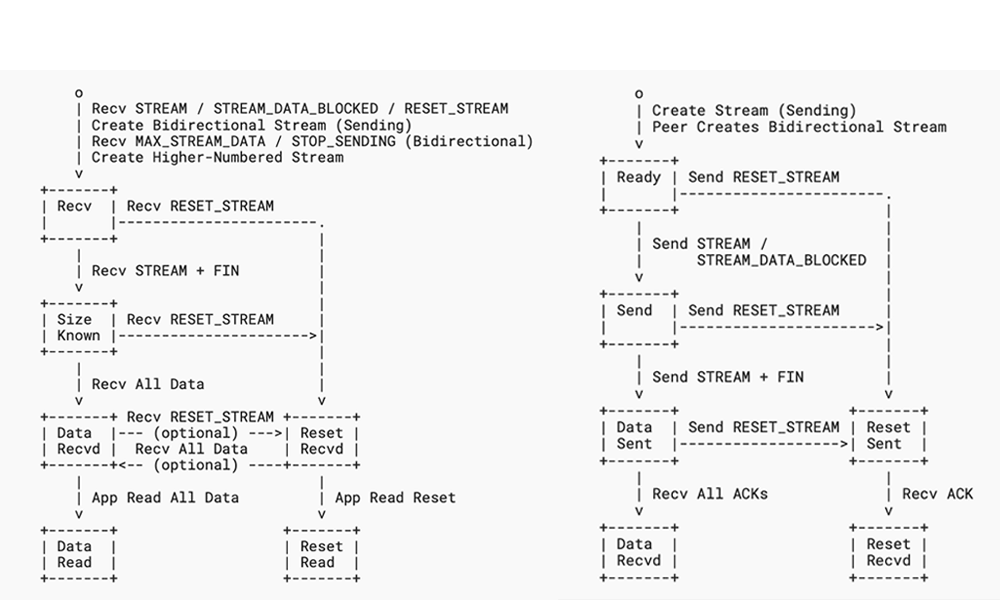
\includegraphics[width=1.0\linewidth]{img/stream_states.png}
  \end{subfigure}
  \caption{Stream States for Receiving (left) and Sending (right) \cite[16-18]{rfc9000}}
  \label{grafik_stream_states}
\end{figure}

The receiving part is initiated upon receiving the first stream frame type for a specific stream ID. For bidirectional streams initiated by the peer, receiving a \\ MAX\_STREAM\_DATA or STOP\_SENDING frame also triggers its creation. In the initial "Recv" state, an arbitrary amount of STREAM or STREAM\_DATA\_BLOCKED frames are handled. Incoming data gets buffered and reassembled for your application. As buffer space frees up with data consumption, MAX\_STREAM\_DATA frames signal the sender to continue transmitting. Receiving a STREAM frame with the FIN bit marks the end of data flow, prompting the transition to the "Size Known" state. Here, MAX\_STREAM\_DATA frames are no longer sent, only potential retransmissions received. Once all data arrives, the stream enters the "Data Recvd" state. Any further STREAM or \\ STREAM\_DATA\_BLOCKED frames can be discarded at this point. From "Data Recvd", the application is able to read the stream data, promting a transition into the terminal "Data Read" state. Receiving a RESET\_STREAM frame in the "Recv" or "Size Known" state transitions the stream to "Reset Recvd," potentially interrupting data delivery. Interestingly, implementations can handle this even if all data has arrived ("Data Recvd") or is still coming ("Reset Recvd"). A RESET\_STREAM doesn't guarantee the sender won't deliver more data. The implementation can choose to:
\begin{enumerate}
    \item Stop delivery, discard unconsumed data, and inform the application about the reset.
    \item Suppress the reset signal if all data is received and buffered, keeping the stream in "Data Recvd."
\end{enumerate}
Finally, receiving the reset notification by the application moves the stream to the terminal "Reset Read" state. \\

When initiating a QUIC stream, the sending part begins in the "Ready" state for both, streams initiated locally and bidirectional streams created by the peer, able to accept application data. This data might be buffered here before transmission. The first sent STREAM or STREAM\_DATA\_BLOCKED frame triggers a transition to the "Send" state. In the "Send" state, the endpoint transmits and retransmits data (STREAM frames) as needed, respecting flow control limits set by the peer and processing \\ MAX\_STREAM\_DATA frames. If blocked by flow control limits, the endpoint sends STREAM\_DATA\_BLOCKED frames. After the application indicates all data is sent, and a STREAM frame with the FIN bit is sent, the stream enters the "Data Sent" state. Here, the endpoint only retransmits data as necessary and ignores flow control and blocked notifications. \\ MAX\_STREAM\_DATA frames might still be received until the final offset arrives. Once all data is acknowledged, the stream enters the terminal "Data Recvd" state. From "Ready," "Send," or "Data Sent," the application can signal abandonment or the endpoint can receive a STOP\_SENDING frame, prompting a RESET\_STREAM frame and transition to the "Reset Sent" state. Alternatively, a RESET\_STREAM frame can be sent as the first stream mention, immediately opening and resetting the stream. Upon acknowledgment of the reset frame, the stream reaches the terminal "Reset Recvd" state.

\subsection{Packets}

QUIC endpoints communicate by exchanging packets. Packets are categorized by their use during connection establishment (Initial, Handshake, Retry) and data transfer (0-RTT, 1-RTT). Encryption levels vary based on packet type, ensuring confidentiality and integrity for sensitive data(\ref{packet_protection}). Version Negotiation and Retry packets are the exception and lack encryption for initial communication as they do not carry sensitive data. Packets are distinguished by an unique identifier. This identifier can range from 0 to $2^{62}-1$  and is encoded as variable sized integer(\ref{variable_sized_integer}) in headers for reduced overhead. During different stages of the connection process, packet numbers are counted separately, resulting in three packet number spaces: Initial, Handshake, and Application. Reusing numbers within a space is strictly prohibited to prevent ambiguity and maintain cryptographic separation. Certain packet types can be coalesced within a single UDP datagram for efficiency, especially while handshaking, but packets within a single datagram must be in increasing encryption level order for proper processing.

QUIC operates under the assumption that the minimum size of an IP packet is at least 1280 bytes, which aligns with the IPv6 standard and is commonly supported by modern IPv4 networks as well. Factoring in the minimum IP header size of 40 bytes for IPv6 and 20 bytes for IPv4, along with a UDP header size of 8 bytes, this yields a maximum datagram size of 1232 bytes for IPv6 and 1252 bytes for IPv4. Consequently, QUIC anticipates that both modern IPv4 and all IPv6 network paths can effectively accommodate its requirements. The minimum allowed packet size is 1200 bytes, therefore packets with not enough available payload must use padding frames to increase their packet size. The maximum packet size is defined as the largest size of UDP payload that can be sent across a network path using a single UDP datagram, but is ultimately governed by flow and congestion control.

A QUIC packet always consists of a header and a payload. Depending on the connection stage, the header structure changes accordingly to ensure optimal efficiency (\ref{headers}). The payload of a QUIC packet consists of individual frames, each with their own header, carrying various data types and instructions.
\begin{enumerate}
    \item \textbf{PADDING} frames (type 0x00) carry no information and may be used to artificially inflate packet size, e.g. initial packets have to be padded to conform to the minimum packet size of 1200 bytes. They do not have to be acknowledged and packets that only contain padding may be used to probe new network paths. \cite[104]{rfc9000}
    \item \textbf{PING} frames (type 0x01) may be used to check reachability of the peer. \cite[105]{rfc9000}
    \item \textbf{ACK} frames (type 0x02 - 0x03) are used to acknowledge packets that have been received and processed. Type 0x02 carries one or more ACK ranges(\ref{ack_range}). If the type is 0x03, ACK frames also carry ECN(\ref{ecn}) counts. They do not have to be acknowledged and packets only containing ACK frames do not count toward bytes in flight for congestion control. \cite[105]{rfc9000}
    \item \textbf{RESET\_STREAM} frames (type 0x04) may be used to abruptly terminate the sending part of a stream. It also contains the application protocol error code. \cite[108]{rfc9000}
    \item \textbf{STOP\_SENDING} frames (type 0x05) may be used to request that a peer ceases transmission on a stream. It also contains the application protocol error code. \cite[109]{rfc9000}
    \item \textbf{CRYPTO} frames (type 0x06) are used to transmit cryptographic handshake messages. They are functionally identical to stream frames except they do not have a stream identifier and they are not flow controlled. \cite[110]{rfc9000}
    \item \textbf{NEW\_TOKEN} frames (type 0x07) contain a token, that is used in the header of an Initial packet for a future connection from the client. \cite[110]{rfc9000}
    \item \textbf{STREAM} frames (type 0x08 - 0x0f) carry stream data. The type is used to encode three different values: the OFF bit (0x04) is set to indicate that there is an Offset field present, the LEN bit (0x02) is set to indicate that there is a Length field present and the FIN bit (0x01) indicates that the frame marks the end of the stream.\cite[111]{rfc9000}
    \item \textbf{MAX\_DATA} \& \textbf{MAX\_STREAM\_DATA} frames (type 0x10 \& 0x11) are used to inform the peer of the maximum amount of data that can be sent on the whole connection or a specific stream. \cite[112, 113]{rfc9000}
    \item \textbf{MAX\_STREAMS} frames (type 0x12 - 0x13) limits the number of concurrent streams the peer is allowed to open (type of 0x12 applies to bidirectional streams and a type of 0x13 applies to unidirectional streams). \cite[114]{rfc9000}
    \item \textbf{DATA\_BLOCKED} \& \textbf{STREAM\_DATA\_BLOCKED} frames (type 0x14 \& 0x15) are used to inform the peer that due to connection-or stream-level flow control limits, no more data can be sent at the time. \cite[114]{rfc9000}
    \item \textbf{STREAMS\_BLOCKED} frames (type 0x16 - 0x17) are used when a sender wishes to open a stream but is unable to do so due to the maximum stream limit set by its peer(0x16 for reaching the bidirectional stream limit, 0x17 for the unidirectional stream limit). \cite[115]{rfc9000}
    \item \textbf{NEW\_CONNECTION\_ID} \& \textbf{RETIRE\_CONNECTION\_ID} frames (type 0x18 \& 0x19) are used to inform the peer about new connection identifiers that may be used or to stop the peer from using specific identifiers in the future. \cite[116, 117]{rfc9000}
    \item \textbf{PATH\_CHALLENGE} \& \textbf{PATH\_RESPONSE} frames (type 0x1a \& 0x1b) are used to check reachability of the peer and for path validation during connection migration. A response can only be sent after receiving a challenge. \cite[118, 119]{rfc9000}
    \item \textbf{CONNECTION\_CLOSE} frames (type 0x1c - 0x1d) are used to notify the peer that the connection is being closed. It also contains an error code and an optional reason phrase. \cite[119]{rfc9000}
    \item \textbf{HANDSHAKE\_DONE} frames (type 0x1e) are used to signal confirmation of the handshake to the client. They do not carry any data.\cite[120]{rfc9000}
\end{enumerate}

\begin{table}[H]
\begin{center}
    \begin{tabular}{| l | l | l |}
    \hline
    \textbf{Type Value} & \textbf{Frame Type Name}  & \textbf{Spec} \\ \hline
    0x00 & PADDING & NP \\ \hline
    0x01 & PING  &  \\ \hline
    0x02 - 0x03 & ACK & NC \\ \hline
    0x04 & RESET\_STREAM &  \\ \hline
    0x05 & STOP\_SENDING &  \\ \hline
    0x06 & CRYPTO &  \\ \hline
    0x07 & NEW\_TOKEN &  \\ \hline
    0x08 - 0x0f & STREAM & F \\ \hline
    0x10 & MAX\_DATA &  \\ \hline
    0x11 & MAX\_STREAM\_DATA &  \\ \hline
    0x12 - 0x13 & MAX\_STREAMS &  \\ \hline
    0x14 & DATA\_BLOCKED &  \\ \hline
    0x15 & STREAM\_DATA\_BLOCKED &  \\ \hline
    0x16 - 0x17 & STREAMS\_BLOCKED &  \\ \hline
    0x18 & NEW\_CONNECTION\_ID & P \\ \hline
    0x19 & RETIRE\_CONNECTION\_ID &  \\ \hline
    0x1a & PATH\_CHALLENGE & P \\ \hline
    0x1b & PATH\_RESPONSE & P \\ \hline
    0x1c - 0x1d & CONNECTION\_CLOSE & N \\ \hline
    0x1e & HANDSHAKE\_DONE &  \\ \hline
    \end{tabular}
\end{center}
\caption{Frame Types \cite[70 - 71]{rfc9000}}
\label{table_frame_types}
\end{table}
The "Spec" column in Table \ref{table_frame_types} provides a summary of any previously mentioned characteristics of the frame type, as indicated by the following symbols.
\begingroup
\renewcommand\labelenumi{(\theenumi)}
\begin{enumerate}
\item[N:] Packets containing only frames with this marking are not ack-eliciting \label{spec_n}
\item[C:] Packets containing only frames with this marking do not count toward bytes in flight for
congestion control purposes \label{spec_c}
\item[P:] Packets containing only frames with this marking can be used to probe new network paths
during connection migration \label{spec_p}
\item[F:] The contents of frames with this marking are flow controlled \label{spec_f}
\end{enumerate}
\endgroup

\subsection{Headers} \label{headers}

In QUIC, packet headers play a crucial role in facilitating efficient communication between endpoints. They serve as the initial segment of each packet and contain key metadata necessary for proper packet processing and routing. QUIC packets can have either a short or a long header, each serving distinct purposes in the communication process. Packets with long headers are primarily used during the connection establishment or reestablishment phase and cryptographic handshake, while short header packets are utilized for ongoing communication sessions to reduce processing overhead.

\subsubsection{Long Header}

Long Header packets contain various fields essential for connection establishment, including the Source Connection ID, Destination Connection ID, Packet Number, and Packet Type. These fields provide information about the endpoints involved, the sequence number of the packet, and its type, facilitating proper routing and processing.

\begin{figure}[htb]
\begin{verbatim}
Long Header Packet {
  Header Form (1) = 1,
  Fixed Bit (1) = 1,
  Long Packet Type (2),
  Type-Specific Bits (4),
  Version (32),
  Destination Connection ID Length (8),
  Destination Connection ID (0..160),
  Source Connection ID Length (8),
  Source Connection ID (0..160),
  Type-Specific Payload (..),
}
\end{verbatim}
    \caption{Base Long Header Format\cite[88]{rfc9000}}
\end{figure}

Depending on the packet type, the type-specific payload changes. There are four different packet types that make use of the long header (Fig. \ref{table_long_header_types}) and which are encoded into the long packet type within the first byte of the long header. Additionally the version negotiation packet makes use of the long header, but is not explicitly encoded due to it being inherently not version specific.

\begin{table}[H]
\begin{center}
    \begin{tabular}{| l | l |}
    \hline
    Type & Name \\ \hline
    0x00 & Initial \\ \hline
    0x01 & 0-RTT \\ \hline
    0x02 & Handshake \\ \hline
    0x03 & Retry \\ \hline
    \end{tabular}
\end{center}
\caption{Long Header Types \cite[90]{rfc9000}}
\label{table_long_header_types}
\end{table}

\textit{Version Negotiation Packets} are identified by the version field having a value of 0. They are not acknowledged and only sent in response to a packet that indicates an unsupported version. Version Negotiation Packets also do not include the Packet Number and Length fields present in other packets that use the long header form. The payload of the Version Negotiation packet is a list of 32-bit versions that the server supports.
\begin{figure}[htb]
\begin{verbatim}
Version Negotiation Packet {
  Header Form (1) = 1,
  Unused (7),
  Version (32) = 0,
  Destination Connection ID Length (8),
  Destination Connection ID (0..2040),
  Source Connection ID Length (8),
  Source Connection ID (0..2040),
  Supported Version (32) ...,
}
\end{verbatim}
    \caption{Version Negotiation Packet\cite[91]{rfc9000}}
\end{figure}

\textit{Initial Header Packets} are sent by clients to a server and have their long packet type set to 0x00 (Fig. \ref{table_long_header_types}). The header contains additional fields for a token, the packet length and the packet number. A token may be used for address validation prior to completing the handshake and is derived from the source connection id which is randomly generated. The reserved bits, the packet number length, the length and the packet number are protected using header protection (\ref{packet_protection}). The packet payload is encrypted separately. Initial packets carry crypto frames and ACKs in either direction. The crypto frames contain the initial client or server hello messages from TLS which are used for the key exchange\cite{rfc9001}.

\begin{figure}[htb]
    \centering      
\begin{verbatim}
Initial Packet {
  Header Form (1) = 1,
  Fixed Bit (1) = 1,
  Long Packet Type (2) = 0,
  Reserved Bits (2),
  Packet Number Length (2),
  Version (32),
  Destination Connection ID Length (8),
  Destination Connection ID (0..160),
  Source Connection ID Length (8),
  Source Connection ID (0..160),
  Token Length (i),
  Token (..),
  Length (i),
  Packet Number (8..32),
  Packet Payload (8..),
}
\end{verbatim}
    \caption{Initial Header Format\cite[92]{rfc9000}}
\end{figure}

\textit{0-RTT Header Packets} are used for instant connection resumption and have their long packet type set to 0x01 (Fig. \ref{table_long_header_types}). Keys for 0-RTT packets are derived during the handshake. 0-RTT packets carry early application data and can be processed if the peer recognizes the sender as a recently turned inactive connection. A handshake can then be carried out while application data is already being exchanged (Sec. \ref{zero_rtt}). 

\begin{figure}[htb]
    \centering      
\begin{verbatim}
0-RTT Packet {
    Header Form (1) = 1,
    Fixed Bit (1) = 1,
    Long Packet Type (2) = 1,
    Reserved Bits (2),
    Packet Number Length (2),
    Version (32),
    Destination Connection ID Length (8),
    Destination Connection ID (0..160),
    Source Connection ID Length (8),
    Source Connection ID (0..160),
    Length (i),
    Packet Number (8..32),
    Packet Payload (8..),
}
\end{verbatim}
    \caption{0-RTT Header Format\cite[94]{rfc9000}}
\end{figure}

\textit{Handshake Header Packets} are used after the initial packets are exchanged and have their long packet type set to 0x02 (Fig. \ref{table_long_header_types}). Handshake packets use their own packet number space, are encrypted using the keys derived from the prior, initial key exchange and carry additional cryptographic handshake messages, including the server certificate and the encrypted TLS extensions\cite{rfc9001}.

\begin{figure}[htb]
    \centering      
\begin{verbatim}
Handshake Packet {
  Header Form (1) = 1,
  Fixed Bit (1) = 1,
  Long Packet Type (2) = 2,
  Reserved Bits (2),
  Packet Number Length (2),
  Version (32),
  Destination Connection ID Length (8),
  Destination Connection ID (0..160),
  Source Connection ID Length (8),
  Source Connection ID (0..160),
  Length (i),
  Packet Number (8..32),
  Packet Payload (8..),
}
\end{verbatim}
    \caption{Handshake Header Format\cite[95]{rfc9000}} 
\end{figure}

\textit{Retry Header Packets} carry an address validation token created by the server and are used if a server wants to perform a retry. Retry packets do not contain any protected fields.

\begin{figure}[htb]
    \centering      
\begin{verbatim}
Retry Packet {
  Header Form (1) = 1,
  Fixed Bit (1) = 1,
  Long Packet Type (2) = 3,
  Unused (4),
  Version (32),
  Destination Connection ID Length (8),
  Destination Connection ID (0..160),
  Source Connection ID Length (8),
  Source Connection ID (0..160),
  Retry Token (..),
  Retry Integrity Tag (128),
}
\end{verbatim}
    \caption{Retry Header Format\cite[96]{rfc9000}} 
\end{figure}

\subsubsection{Short Header}

Short Header packets, on the other hand, contain a reduced set of fields compared to Long Header packets, including only the Connection ID and Packet Number. This streamlined header format is employed for more efficient transmission during established communication sessions, reducing overhead and improving performance. Encrypted fields include the reserved bits, the key phase, the packet number length, the packet number and the packet payload. They are encrypted and decrypted using 1-RTT keys derived during the prior handshake.

\begin{figure}[htb]
    \centering      
\begin{verbatim}
1-RTT Packet {
  Header Form (1) = 0,
  Fixed Bit (1) = 1,
  Spin Bit (1),
  Reserved Bits (2),
  Key Phase (1),
  Packet Number Length (2),
  Destination Connection ID (0..160),
  Packet Number (8..32),
  Packet Payload (8..),
}
\end{verbatim}
    \caption{Base Short Header Format\cite[98]{rfc9000}}
\end{figure}

The latency spin bit facilitates passive monitoring of latency from various observation points along the network path throughout a connection's lifespan. Upon receiving the spin value, the server mirrors it, while the client toggles it after one round-trip time (RTT). By measuring the time elapsed between successive spin bit toggles, on-path observers can estimate the end-to-end RTT of the connection. The presence of the spin bit is confined to 1-RTT packets, as the initial RTT of a connection can be calculated by observing the handshake.

\subsection{Header and Packet Protection} \label{packet_protection}

QUIC, similarly to TLS over TCP, uses keys derived from the TLS handshake to encrypt and decrypt packets, utilizing the AEAD algorithm negotiated by TLS. Depending on their type, QUIC packets employ varying levels of protection:
\begin{itemize}
    \item \textbf{Version Negotiation Packets} lack cryptographic protection entirely.
    \item \textbf{Retry Packets} employ AEAD\_AES\_128\_GCM (\ref{aead}) to prevent inadvertent tampering and restrict the entities capable of producing a valid Retry.
    \item \textbf{Initial Packets} utilize AEAD\_AES\_128\_GCM with keys derived from the Destination Connection ID field of the client's initial Initial packet and a publicly available salt in RFC 9001 \cite[20]{rfc9001}.
    \item \textbf{Other Packets} boast robust cryptographic protections ensuring confidentiality and integrity, utilizing keys and algorithms negotiated by TLS.
\end{itemize}

QUIC employs separately derived keys for header and payload protection, ensuring confidentiality for specific header fields not exposed to on-path elements. Header protection extends to the least significant bits of the first byte and the Packet Number field. The header protection key remains constant throughout the connection, allowing header protection to be utilized continuously. Packet protection keys in QUIC are derived in a manner akin to TLS's derivation of record protection keys. Theses keys are computed from the TLS secrets using the Key Derivation Function (KDF) provided by TLS. For instance, in TLS 1.3, the Hash-based KDF-Expand-Label function is employed with a hash algorithm agreed on during the handshake and labels provided by the RFC \cite[20]{rfc9001}. During 1-RTT communication, either endpoint may initiate a key update at any time (see sec. \ref{security}).

\subsection{Flow Control} \label{flow_control}

QUIC uses a limit-based flow control scheme to prevent buffer overflows and ensure smooth data delivery. This system operates on two levels:
\begin{enumerate}
    \item \textbf{Stream Flow Control} manages individual streams, preventing any single stream from monopolizing the receiver's buffer. In turn, receivers advertise the maximum data they can accept for each stream and senders must adhere to these limits and stop sending when they reach the advertised amount.
    \item \textbf{Connection Flow Control} provides an overall limit for the entire connection, ensuring the receiver's buffer doesn't become overloaded. Receivers advertise the total data they can accept for all streams combined and senders must adhere to this limit as well, distributing data across streams within the allowed quota.
\end{enumerate}
A receiver must set initial limits for all streams through transport parameters during the handshake. Subsequently, a receiver sends MAX\_STREAM\_DATA frames or MAX\_DATA frames to the sender to advertise larger limits. Flow control limits are dynamic, adapting to network conditions and buffer availability. Receivers can decrease the window size upon congestion or increase it when buffer space permits, ensuring efficient resource utilization.

\subsection{Congestion Control} \label{congestion_control}

While QUIC's loss detection and congestion control algorithms share similarities with TCP, underlying protocol differences lead to some
variations\cite{rfc9002}:

\begin{itemize}
    \item Clearer Loss Epochs: QUIC defines a loss epoch starting when a packet is lost and ending with the acknowledgement of any subsequent
    packet. This contrasts with TCP, where epochs might linger for multiple round-trips due to gaps in the sequence number space.
    \item No Reneging on Acknowledgements: QUIC acknowledgements, similar to TCP's Selective Acknowledgements (SACKs), are permanent, simplifying
    implementation and reducing memory usage on the sender side.
    \item Explicit Correction for Delayed Acknowledgements: QUIC accounts for delays between packet reception and acknowledgement, allowing for
    more accurate round-trip time (RTT) estimations.
    \item Probe Timeout (PTO) Replaces RTO and TLP: QUIC utilizes a PTO timer based on TCP's RTO concept but incorporates the peer's expected
    acknowledgement delay for a more precise timeout. Unlike TCP, QUIC doesn't collapse the congestion window upon PTO expiration for a
    single lost packet. This avoids unnecessary congestion control reductions.
    \item Minimum Congestion Window of Two Packets: QUIC recommends a minimum congestion window of two packets to avoid potential delays caused
    by waiting for a single packet acknowledgement after loss.
    \item Handshake Packets Treated as Regular Packets: QUIC handles lost handshake packets just like any other data loss, unlike TCP's approach
    of treating them as a sign of persistent congestion.
\end{itemize}

QUIC has two ways to detect packet loss, either by a missing acknowledgement or by timeout of the Probe Timeout (PTO) which is initialized
whenever an ack-eliciting packet is sent (see Sec. \ref{loss_detection_recovery}).

\subsubsection{Estimating Round Trip Times}

An RTT sample is generated upon receiving an acknowledgement (ACK) frame that meets two criteria:
First, It acknowledges the largest packet number not previously acknowledged.
Second, At least one of the newly acknowledged packets triggered an acknowledgement (ack-eliciting frame).
The RTT sample (\inlinecode{latest\_rtt}) is calculated by measuring the time elapsed since the largest acknowledged packet was sent.

Additionally, the minimum rtt (\inlinecode{min\_rtt}) is tracked. The \inlinecode{min\_rtt} represents the sender's observation of the absolute
minimum RTT for the connection. It is initialized to the first received RTT sample (\inlinecode{latest\_rtt}). Subsequent samples are compared
to \inlinecode{min\_rtt}, and the lower value is retained.

The Smoothed RTT (\inlinecode{smoothed\_rtt}) represents an exponentially weighted moving average of RTT samples, providing a more stable
estimate than individual samples. The RTT Variation \inlinecode{rttvar} reflects the degree of fluctuation in observed RTT samples.

While calculating the rtt times, a sample may be adjusted based on acknowledgement delays reported by the peer. Furthermore, during the
handshake, QUIC might ignore peer-reported delays or limit them to a maximum value to avoid
biasing the RTT estimate. Lastly, QUIC may account for local processing delays (e.g., decryption) when calculating RTT samples.

\subsubsection{Algorithms}

The sender-side Congestion Control Algorithm specified in RFC 9002\cite[17]{rfc9002} shares similarities with TCP's
NewReno\cite[]{rfc6582} but presents only a suggestion. Implementations have the flexibility of choosing their own algorithm such as
Cubic\cite[]{rfc8312} or add improvements like HyStart++\cite[]{rfc9406}.

\begin{figure}[h]
    \centering
    \begin{subfigure}[b]{1.0\textwidth}
      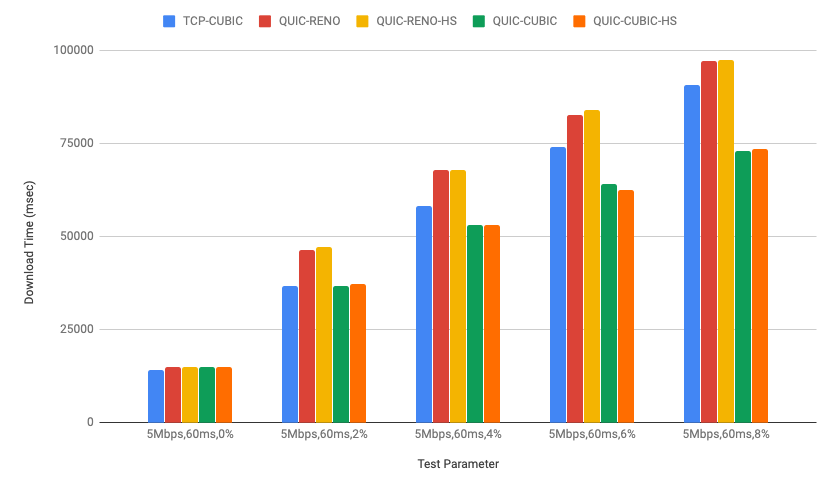
\includegraphics[width=1.0\linewidth]{img/cc}
    \end{subfigure}
    \caption{Comparison of different CC Algorithms (HS = HyStart++) \cite[]{ccgraphic}}
    \label{cc_comparison}
\end{figure}

QUIC uses a congestion window to limit the number of bytes in flight (unacknowledged packets) at any given time. A sender cannot
transmit a packet that would exceed the congestion window which is adjusted dynamically based on network conditions. QUIC defines
three congestion control states: Slow Start, Recovery, and Congestion Avoidance. Slow Start is used initially, the window grows
exponentially to quickly probe the network capacity. The recovery is entered upon packet loss or ECN increase. The window is
then reduced and slow start is re-initiated. During Congestion Avoidance, the window is gradually increased using Additive
Increase Multiplicative Decrease (AIMD) to avoid further congestion.

QUIC can detect persistent congestion when packet loss persists for a certain duration. Upon detection, the congestion window is
drastically reduced to a minimum value similar to TCP's response on a timeout.

QUIC recommends pacing packets to avoid overwhelming the network with bursts. Pacing algorithms spread packets evenly over time
based on the congestion window and RTT (Round Trip Time). ACK packets (acknowledgments) are exempt from pacing to ensure timely delivery.
If the sender has data to send but the number of bytes in flight is less than the window (due to application limitations or flow control),
the window won't be increased. A pacing mechanism might also delay sending packets, leading to underutilization. However, the sender
shouldn't be considered application limited in this case.

Overall, QUIC's congestion control aims to achieve efficient data transfer by dynamically adjusting the sending rate based on network
conditions while avoiding congestion collapse

\subsection{0-RTT Connection} \label{zero_rtt}

The 0-RTT (Zero Round-Trip Time) connection handshake in QUIC is a feature designed to reduce latency by allowing clients to send
data in the very first packet of a connection, without waiting for any round trips to complete. A server may choose to enable it
and notifies the client in the initial cryptographic handshake. It is typically used when a client has previously established a
connection with a server and has cached the session state, including cryptographic keys and other parameters, and wants to
reestablish the connection, for example when loading a website the client has visited shortly before. This however implicates
that clients and servers need to manage cached session data securely.

To initiate a 0-RTT connection, the client sends a packet with a long header of type 0x01 (\ref{table_long_header_types}) and
includes all cached session data from the previous connection. Upon receiving the client's initial packet, the server attempts
to decrypt and validate the cached session data. If successful, it can immediately process and respond to the client's request,
without requiring any additional round trips. To ensure security, the cached session data is encrypted using keys derived from
the previous session's cryptographic handshake. If the server cannot successfully validate the cached session data (e.g., due to
expiration, tampering, or other reasons), it falls back to a regular full handshake process, which involves additional round
trips for establishing a new session.

By allowing the client to send data in the first packet, the 0-RTT handshake significantly reduces the connection establishment
latency, leading to faster transmission of data. Additionally, minimizing round trips and accelerating the connection setup process
improves network resource utilization and reduces congestion, benefiting both clients and servers. Allowing application data before
properly securing the connection however introduces a potential security risk. Therefore applications may limit the data a 0-rtt can
access, for example many HTTP/3 implementations only allow GET request prior to the completed 0-rtt handshake.

\subsection{Connection Migration} \label{connection_migration}

As Quic was designed with todays technology in mind, a key feature was its ability to remove the reliance on a never changing network
interface during communication. For example, if a device from which a QUIC session has been established would leave the home WIFI
network with his or her mobile phone and go outside, the mobile phone would log into the nearest Radio Access Node. A traditional TCP
connection would collapse under these circumstances because the host address would change.
Therefore the connection would have to be re-initiated from scratch, resulting in significant time and processing overhead. QUIC
solves this problem by introducing a connection identifier which is not bound to any interface and only refers to the connection
itself. Therefore a reconnecting host can still identify itself and resume the session on a new network path.

During connection migration, two processes play a crucial role:
\begingroup
\renewcommand\labelenumi{(\theenumi)}
\begin{enumerate}
\item \textbf{Path Validation} assesses the quality, reliability, and suitability of a network path for communication. It verifies
whether a new network path, including its latency, packet loss characteristics, and other properties, is suitable for transmitting
data. Path validation often involves sending probing packets along the new network path and analyzing the responses to determine its
characteristics and suitability for data transmission.\cite[46]{rfc9000} \label{path_validation}
\item \textbf{Address Validation} verifies the legitimacy and ownership of a peer's address. Address validation typically
involves checking cryptographic properties or exchanging validation tokens to ensure that the IP address is genuinely associated
with the intended peer. \cite[42]{rfc9000} \label{address_validation}
\end{enumerate}
\endgroup

If a QUIC connection is migrated onto a new network path, the new network path may get validated first through the use of probing
packets. The migration is initiated with the first packet containing non-probing frames. If an endpoint receives a packet with a
known connection identifier from an address which it does not recognize, it must perform address validation first before sending
any data over the new path. If the address validation is successful, connection identifiers are renewed and congestion control and
the round-trip time estimation are reset for the new path. QUICs Ack-based loss detection will detect and resend any packets that
may have gotten lost during connection migration or due to packet loss in the network to achieve a graceful resumption of the
previous connection.

\subsubsection{Preferred Address}

Servers can communicate a preferred address to clients by including it in the \\ quic\_transport\_parameters extension inside the initial handshake messages allowing for migration to a more preferred address after the handshake. Clients select the preferred address, validate it, and initiate migration accordingly. This implies a setup in which a QUIC server functions as a load balancer, handling only handshakes and distributing incoming connections to other servers \footnote{\url{https://github.com/envoyproxy/envoy/issues/12651}}.

\section{Connection}

Having explored the complex architectural foundations of QUIC in the previous chapter, we now shift our focus to the heart of the
protocol: the connection process. This critical process dictates how clients and servers initiate communication, negotiate security
parameters, and ultimately exchange data securely. Unlike the traditional three-way handshake of TCP, QUIC adopts a more streamlined
and robust approach, incorporating TLS directly and allowing for connection migration or zero round-trip time (0-RTT) handshakes, where
application data may be sent before the handshake is completed.

In traditional TCP with TLS (Transport Layer Security), the handshake typically spans three round-trip times (3-RTT)
(Fig. \ref{handshake_comparison}). During this process, the client initiates the connection by sending a SYN packet to the server,
which responds with a SYN-ACK packet. Upon receiving the SYN-ACK, the client sends an ACK packet, completing the handshake.
Following this, TLS negotiation occurs, involving multiple exchanges of handshake messages to establish cryptographic parameters
and keys for secure communication. While effective in ensuring security, the 3-RTT handshake introduces latency due to the multiple
round trips required, impacting the connection's responsiveness, especially over high-latency networks.

In contrast, QUIC introduces a more streamlined approach to handshaking, aiming to minimize latency and improve performance.
QUIC's 1-RTT handshake (Fig. \ref{handshake_comparison}) achieves this by combining the connection establishment and cryptographic
negotiation into a single round trip. The client's initial packet contains cryptographic parameters and keys. Upon receiving this
packet, the server decrypts the information, verifies the client's authenticity, and responds with its own cryptographic parameters
and keys, allowing secure communication to commence. By consolidating these steps into a single round trip, QUIC significantly
reduces handshake latency compared to TCP + TLS.

Moreover, QUIC introduces the even more efficient 0-RTT handshake, aimed at further minimizing latency for subsequent connections
between known peers. In the 0-RTT handshake, a client caches cryptographic parameters and keys from a previous connection with the
server. Upon reconnecting, the client is able to send encrypted application data within the first packet. If the server can
validate the client's authenticity, it is able to resume the previous session, while redoing the handshake simultaneously, saving one
round trip. This approach eliminates the need for the initial handshake rountrip, enabling instantaneous connection reestablishment. 
However, it comes with security considerations, as replay attacks and potential cryptographic vulnerabilities need to be addressed
to ensure the integrity and confidentiality of the communication. In the following subchapters the different types of QUIC handshakes
are presented in more detail.

\begin{figure}[h]
  \centering
  \begin{subfigure}[b]{1.0\textwidth}
    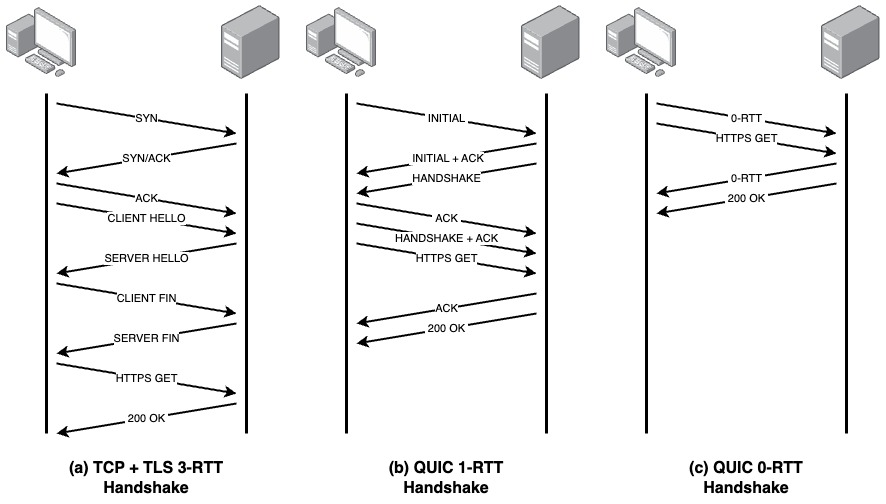
\includegraphics[width=1.0\linewidth]{img/handshake_illustration.jpg}
  \end{subfigure}
  \caption{Comparison between handshakes}
  \label{handshake_comparison}
\end{figure}

\subsection{1-RTT Handshake}

If a client wishes to initiate a connection to a QUIC server, it starts by sending the initial packet. An initial packet has a long
header of type 0x00 (\ref{table_long_header_types}) and carries a source connection id chosen by the client and a randomly generated
destination connection id. The payload contains a crypto frame which holds the TLS Client Hello and additional padding bytes to conform
to the minimum packet size of 1200 bytes. The Client Hello follows the TLS 1.3 specification \cite{rfc8446} but has been specially
modified for QUIC in rfc 9001 \cite{rfc9001}. The client offers a set of cipher suites, shares the public key, provides the used 
application layer protocol and specifies the clients transport parameters for QUIC. The application layer protocol chosen by the client
is encoded as the UTF-8 representation of its name string. IANA keeps a list of registered and standardised protocol codes. Proprietary
protocols may be used if the client and the server use the same encoded string. The transport parameters include various stream limits,
the initial source connection id also used in the header, a stateless reset token and time limits for later acknowledgements.
QUIC transport parameters are fixed and apply for possible retry and 0-rtt packets. The provided source connection ids from the
transport parameters and the packet header must be identical to be deemed authenticated. Packet payloads from the initial packet
number space are encrypted using a key derived from the randomly generated connection id. Header protection is always applied
after packet protection because the first 16 bytes from the already encrypted payload are sampled and used as additional input
for the encryption algorithm.

Upon receiving an initial packet from a client, the server first performs a partial header decode in which all unencrypted header data
is read. Using the provided destination connection id and the public salt value from the rfc, the server can now generate the key
pair to decrypt the packet. After decrypting the packet, the packet number and the payload can now be processed. The server
can now authenticate the source connection id by comparing it to
the source connection id provided in the QUIC transport parameters. It chooses one of the provided cipher suites, verifies that
the specified application layer protocol is supported and prepares its own transport parameters. If the server does not support
the specified protocol, the connection is immediately terminated.
The servers transport parameters include all parameters it received from the client with the servers' values alongside the original
destination connection id it received and a newly generated source connection id which replaces the original destination connection
id (Fig.\ref{handshake_cids}). The server is now able to construct its answer which includes a crypto frame with the returning TLS
Server Hello and an acknowledgement frame to confirm the successful receival of the initial packet. The Server Hello contains all
the negotiated upon parameters and the servers public key.

\begin{figure}[htb]
    \centering      
\begin{verbatim}
Client                                                     Server

Initial: DCID=S1, SCID=C1 ->
                                     <- Initial: DCID=C1, SCID=S3
                                ...
1-RTT: DCID=S3 ->
                                                <- 1-RTT: DCID=C1
\end{verbatim}
    \caption{Use of connection ids during Handshake\cite[38]{rfc9000}}
    \label{handshake_cids}
\end{figure}

When building the outgoing packet header, the received source connection ID becomes the destination connection ID, while the
self-generated source connection ID replaces the provided destination connection ID. The packet and its header is then encrypted
using the previously derived initial keys associated with the original destination ID. The Server now has the option to consolidate
multiple packets into a single UDP datagram, giving it the opportunity to directly provide the first handshake packet, drastically
increasing efficiency. In order to do so, the server upgrades the packet number space to the handshake space. Subsequently,
the new keys can be computed utilizing the data extracted from the client hello. A handshake packet features a long header of
type 0x03 (\ref{table_long_header_types}), and also carries crypto frames and acknowledgments, albeit with enhanced security
measures. The server can now fill the first handshake packet with additional TLS data like the encryption extensions, the server
certificate and the server certificate verify. The packet is then also encrypted and directly appended to the initial packet. It's
imperative that coalesced packets maintain an ascending order in the packet number space to ensure that the necessary information
is processed in the correct sequence.

\begin{figure}[htb]
    \centering      
\begin{verbatim}
Client                                                     Server

Initial[0]: CRYPTO[CH] ->

                                    Initial[0]: CRYPTO[SH] ACK[0]
                          Handshake[0]: CRYPTO[EE, CERT, CV, FIN]
                                    <- 1-RTT[0]: STREAM[1, "..."]

Initial[1]: ACK[0]
Handshake[0]: CRYPTO[FIN], ACK[0]
1-RTT[0]: STREAM[0, "..."], ACK[0] ->

                                             Handshake[1]: ACK[0]
            <- 1-RTT[1]: HANDSHAKE_DONE, STREAM[3, "..."], ACK[0]
\end{verbatim}
    \caption{Example 1-RTT Handshake\cite[35]{rfc9000}}
    \label{example_handshake}
\end{figure}

Figure \ref{example_handshake} offers an overview of the previously described 1-RTT handshake process. Each line illustrates a
QUIC packet, presenting the packet type and packet number followed by the contained frames. For example,
the initial packet is categorized as "Initial," featuring packet number 0 and comprising a CRYPTO frame that carries the Client Hello.
The complete handshake requires a minimum of four UDP datagrams (within the protocol's limitations, such as congestion
control and flow control), using coalescing packets. For instance, the server's initial UDP datagram includes an initial packet,
a handshake packet, and possible "0.5-RTT data" enclosed within a fully protected 1-RTT packet.

The handshake completes when all initial and all handshake packets have been acknowledged by the opposing endpoint.

\subsection{Transmitting Data}

In an established QUIC connection, data is continuously exchanged between the client and server over the established connection.
Each endpoint sends and receives application data using streams (\ref{multiplexing_w_streams}). Each packet is individually encrypted
and authenticated using the negotiated keys, ensuring data integrity and security. During the life-span of the connection, both
parties adjust their congestion control (\ref{congestion_control}) parameters to optimize data transmission based on network conditions.
This ensures efficient utilization of available bandwidth while helping to avoid congestion and packet loss.

In the event of packet loss, QUIC employs mechanisms such as retransmission and adjusts its congestion control algorithms to
recover from the loss and maintain data integrity (\ref{error_handling_recovery}). Furthermore, the connection may adapt to changes
in network conditions (\ref{flow_control}) or migrate to a new network interface (\ref{connection_migration}).

\subsection{Connection Termination}

A connection can terminate in three different ways:

\begingroup
\renewcommand\labelenumi{(\theenumi)}
\begin{enumerate}
\item \textbf{Idle Timeout:} If specified in the transport parameters, a connection is closed and its state discarded if it remains
idle for longer than the minimum of the max\_idle\_timeout value negotiated upon by both endpoints. Endpoints restart their idle timers
upon receiving and processing packets from their peers or when sending specific acknowledgments. \cite[57]{rfc9000} \label{idle_timeout}
\item \textbf{Immediate Close:} An endpoint can terminate the connection abruptly by sending a CONNECTION\_CLOSE frame, causing all streams to immediately close. After sending this frame, the endpoint enters a closing state, while the receiving endpoint enters a draining state to ensure proper closure. \cite[58]{rfc9000} \label{immediate_close}
\item \textbf{Stateless Reset:} In scenarios where an endpoint loses or is unable to confirm a connection state, it may send a
stateless reset as a last resort. This involves sending a packet containing a reset token that, when received by the peer,
prompts immediate termination of the connection. Stateless resets are used when an endpoint cannot properly continue the connection
due to crashes or outages. \cite[61]{rfc9000} \label{stateless_reset}
\end{enumerate}
\endgroup

In addition to the primary methods of connection termination, there are several important procedures related to handling connection termination scenarios effectively.

\begingroup
\renewcommand\labelenumi{(\theenumi)}
\begin{enumerate}
\item \textbf{Liveness Testing:} When a connection is at risk of timing out, endpoints can send PING frames or other acknowledgment-eliciting frames to test the connection for liveness. This helps ensure that connections are not erroneously terminated due to perceived inactivity. \label{liveness_testing}
\item \textbf{Deferring Idle Timeout:} In situations where an endpoint expects response data but cannot send application data, there may be a need to defer the idle timeout. This option allows the endpoint to periodically send PING frames to restart the idle timeout period, preventing premature closure of the connection while waiting for further activity. \label{deferring_idle_timeout}
\item \textbf{Detecting and Preventing Looping:} Stateless Resets are designed to be indistinguishable from valid packets, but precautions must be taken to prevent looping scenarios. Endpoints should ensure that every Stateless Reset they send is smaller than the packet that triggered it, and limits on the number of Stateless Resets sent can prevent infinite exchanges that could disrupt network operations. \label{detecting_and_preventing_looping}
\item \textbf{Stateless Reset Token Management:} Stateless reset tokens are used as a last resort for terminating connections when
state is lost. Endpoints use pseudorandom functions with static keys and connection IDs to generate tokens, ensuring that they are unique and secure. It's crucial to manage these tokens carefully to prevent misuse or unintended consequences, such as denial-of-service attacks. \label{stateless_reset_token_management}
\end{enumerate}
\endgroup

By following the specified procedures, QUIC implementations can manage connection termination scenarios effectively, ensuring the stability and reliability of the protocol in various network conditions.

\section{Error Handling and Recovery} \label{error_handling_recovery}

During an active connection, errors may occur at any given time. Error handling and recovery are critical aspects of any network
protocol, ensuring
reliability of communication in events such as packet loss, network congestion, and endpoint implementation failures. QUIC employs
many error
handling and recovery mechanisms to address potential issues and mitigate the impact of errors during data transmission, for
example QUIC's loss detection mechanisms, which enable the protocol to identify and respond to packet loss. Additionally,
QUIC can detect and handle numerous other errors, propagate error information between endpoints and handle exceptional
conditions such as protocol violations and connection failures.

\subsection{Loss Detection and Recovery} \label{loss_detection_recovery}

Like its predecessor TCP, QUIC uses an acknowledgement-based loss detection approach to ensure reliability while transferring
data. Packets are identified by their sequentially increasing packet numbers. A packet must not be acknowledged until it has been
successfully decrypted and all frames contained in the packet have been processed. A packet is ack-eliciting
if it contains at least one other frame except acknowledgements itself, PADDING or CONNECTION\_CLOSE. Each acknowledgment is
sent inside an ACK frame, encoded either as type 0x02 or type 0x03, carry acknowledgment ranges to identify acknowledged packets.
Additionally, type 0x03 ACK frames include information about Explicit Congestion Notification (ECN) feedback. The content of ACK
frames, as depicted in Figure \ref{ack_frame}, contain the Type, Largest Acknowledged, ACK Delay, ACK Range Count, First ACK
Range, ACK Ranges, and optionally ECN Counts. 

\begin{figure}[htb]
    \centering      
\begin{verbatim}
ACK Frame {                            ACK Range {
  Type (i) = 0x02..0x03,                   Gap (i),
  Largest Acknowledged (i),                ACK Range Length (i),
  ACK Delay (i),                       }
  ACK Range Count (i),        
  First ACK Range (i),        
  ACK Range (..) ...,         
  [ECN Counts (..)],          
}
\end{verbatim}
    \caption{ACK Frame (left) \cite[106]{rfc9000}, ACK Range (right) \cite[107]{rfc9000}}
    \label{ack_frame}
\end{figure}

Largest Acknowledged represents the highest packet number the peer is acknowledging. The ACK Delay field encodes the acknowledgment delay in microseconds. Moreover, ACK frames may contain an arbitrary number of additional ACK Ranges, which consist of alternating Gap and ACK Range Length values in descending packet number order. Each ACK range acknowledges a contiguous range of packets. The Gap field signifies the number of contiguous unacknowledged packets preceding the packet number one lower than the smallest in the preceding ACK Range. The ACK Range Length field indicates the number of contiguous acknowledged packets preceding the largest packet number. Furthermore, if the ACK frame type is 0x03, ECN feedback is included, providing insights into the number of packets received with specific ECN codepoints (ECT0, ECT1, ECN-CE) in the packet number space of the ACK frame. ECN counts are maintained separately for each packet number space. Figure \ref{ack_frame_example} shows an example ACK frame for a provided number of successfully received packets.

\begin{figure}[htb]
    \centering
\begin{verbatim}
Received packet numbers: [5, 6, 7, 8, 10, 11, 12, 13, 14, 17, 18, 19, 20]

ACK Frame {
  Type = 0x02,
  Largest Acknowledged = 20,
  ACK Delay (i),  //ommitted for this example
  ACK Range Count = 2,
  First ACK Range = 3,        
  Gap = 2,
  Ack Range Length = 5,
  Gap = 1,
  Ack Range Length = 4,
}
\end{verbatim}
    \caption{Example ACK frame}
    \label{ack_frame_example}
\end{figure}

An endpoint should attempt to include an ACK frame with every packet sent to aid in timely loss detection at the peer. 

QUIC employs two types of thresholds for determining packet loss. First, packet number-based thresholds compare the sequence
number of in-flight packets with the acknowledged packet. If the in-flight packet's sequence number is smaller than the
acknowledged packet by a agreed upon threshold ($x - t$), it is marked as lost. Second, time-based thresholds assess the time
elapsed since the acknowledged packet was sent. If an in-flight packet was sent before a certain time threshold ($t - t_{0}$), it is declared lost. These thresholds allow for some tolerance for packet reordering and aim to prevent unnecessary retransmissions without compromising congestion control performance.

To detect packet losses, QUIC initializes a Probe Timeout (PTO) timer whenever a packet requiring acknowledgment is sent. This timer incorporates factors such as smoothed network RTT, RTT variation, and maximum acknowledgment delay. When the PTO timer expires, the sender sends a new packet as a probe to elicit acknowledgments, potentially retransmitting some in-flight data to minimize redundant retransmissions.

QUIC packets that are determined to be lost are not retransmitted whole; instead, the information carried in lost packets is sent again in new frames which are packed into new outgoing packets, each assigned new packet numbers unrelated to the lost ones. Retransmitted data can still be contextualized by examining the offset parameter in the frame headers. This process ensures reliable ordered byte-stream delivery, akin to TCP's functionality, despite packet loss occurrences.

\subsection{Protocol or Application Errors}

One key aspect of QUIC's error handling is its reliance on error codes and connection states to communicate and manage errors effectively. When errors occur, QUIC endpoints may close the connection using the defined transport error codes, allowing the peer to understand the nature of the problem. These error codes cover a wide range of scenarios, including connection establishment failures, packet decryption errors, and protocol violations, providing comprehensive diagnostic information to facilitate error resolution. QUIC transport error codes can be used in a CONNECTION\_CLOSE frame with a type of 0x1c.

\begin{table}[H]
\begin{center}
    \begin{tabular}{| l | l | p{75mm} |}
    \hline
    Error Code & Name & Description \\ \hline
    0x00 & NO\_ERROR & An endpoint uses this with CONNECTION\_CLOSE to signal that the connection is being closed abruptly in the absence of any error. \\ \hline
    0x01 & INTERNAL\_ERROR & The endpoint encountered an internal error and cannot continue with the connection. \\ \hline
    0x02 & CONNECTION\_REFUSED & The server refused to accept a new connection. \\ \hline
    0x03 & FLOW\_CONTROL\_ERROR & An endpoint received more data than it permitted in its
advertised data limits. \\ \hline
    0x04 & STREAM\_LIMIT\_ERROR & An endpoint received a frame for a stream identifier that exceeded its advertised stream limit for the corresponding stream type. \\ \hline
    0x05 & STREAM\_STATE\_ERROR & An endpoint received a frame for a stream that was not in a state that permitted that frame. \\ \hline
    0x0a & PROTOCOL\_VIOLATION & An endpoint detected an error with protocol compliance that was not covered by more specific error codes. \\ \hline
    0x0c & APPLICATION\_ERROR & The application or application protocol caused the connection to
be closed. \\ \hline
    0x0f & AEAD\_LIMIT\_REACHED & An endpoint has reached the confidentiality or integrity limit
for the AEAD (\ref{aead}) algorithm used by the given connection. \\ \hline
    0x10 & NO\_VIABLE\_PATH & An endpoint has determined that the network path is incapable of supporting QUIC. \\ \hline
    \end{tabular}
\end{center}
\caption{A Selection of QUIC Transport Error Codes \cite[121]{rfc9000}}
\label{tabelle_transport_error_codes}
\end{table}

In addition to handling protocol-level errors, QUIC also provides a way for applications to define and use their own error codes.
This enables applications to gracefully handle errors such as resource
exhaustion, application-layer protocol violations, or user-defined conditions, enhancing the overall robustness and resilience
of QUIC-based applications. Application-defined error codes can be utilized for various purposes, including the RESET\_STREAM
frame, the STOP\_SENDING frame, and the CONNECTION\_CLOSE frame with a type of 0x1d (\ref{table_frame_types}).

\section{Security} \label{security}

QUIC security is based on a threat model described in existing security considerations, addressing both passive and
active attacks. Passive attackers can intercept packets, while active attackers can manipulate or inject packets into the network,
potentially intercepting packet routes.
Attackers are further categorized as on-path or off-path, depending on their ability to intercept and manipulate packets. On-path
attackers have direct access to packet routes, enabling various forms of interference, including modification and packet dropping.
Off-path attackers, though unable to directly manipulate packet routes, can still inject packets into the network.
The handshake process in QUIC leverages TLS 1.3, inheriting its cryptographic properties and protections like continuously renewing
keysets or different protection levels for different packet types. Any compromise in the TLS handshake could impact the security
guarantees provided by QUIC. Moreover, QUIC incorporates defenses against denial-of-service (DoS) attacks during the handshake,
such as address validation and server-side DoS prevention mechanisms.
Packet protection in QUIC employs authenticated encryption, ensuring the integrity and confidentiality of transmitted data.
While only on-path attackers can passively observe packets, active attacks are mitigated by cryptographic protection,
preventing unauthorized modifications to packet payloads.
Connection migration capabilities in QUIC allow endpoints to transition between network paths while maintaining security. Path
validation mechanisms help mitigate address spoofing attacks, limiting the impact of packet interception and manipulation.

\subsection{Security Considerations by QUIC}

In its specification, QUIC lists several considerations which had an impact on its design, including known attacks and countermeasures\cite{rfc9000}. These encompass but are not limited to the following:

\begin{itemize}
    \item \textbf{Amplification Attacks} exploit an address validation token to spoof the same address for a 0-RTT connection. An attacker is then able to direct a server to send data towards a victim endpoint. Mitigation involves limiting token usage and lifetime.
    \item \textbf{Optimistic ACK Attacks} involve an endpoint acknowledging packets which it did not receive and can lead to the congestion controller permitting excessive sending rates. Endpoints may close the connection upon detecting this behavior.
    \item \textbf{Explicit Congestion Notification Attacks} are performed by manipulating ECN fields in the IP Header to influence the sender's rate of transmission. Therefore endpoints may ignore ECN fields until at least one QUIC packet from the IP packet is processed without errors.
    \item \textbf{Targeted Attacks by Routing} can be prevented by limiting the ability of an attacker to target a new connection to a particular server instance.
\end{itemize}

\subsection{Tested Attacks}

\begin{table}[H]
\begin{center}
    \begin{tabular}{| p{40mm} | l | p{60mm} | l |}
    \hline
    \textbf{Attack Name} & \textbf{Type} & \textbf{Impact} & \textbf{Reference} \\ \hline
    Source-Address Token Replay Attack & Replay & Server DoS & \cite{quic_security_2} \\ \hline
    Packet Manipulation Attack & Manipulation & Connection establishment failure / server load & \cite{quic_security_1} \cite{quic_security_2} \\ \hline
    Crypto Stream Offset Attack & Manipulation & Connection establishment failure & \cite{quic_security_1} \\ \hline
    Randomized Packet Fuzzing & Fuzzing & Possible server crash & \cite{quic_security_3} \\ \hline
    \end{tabular}
\end{center}
\caption{A selection of tested attacks against QUIC}
\label{table_tested_attacks}
\end{table}

\subsubsection{Source-Address Token Replay Attack}

The Source-Address Token Replay Attack exploits the vulnerability of the initial token, which is designed to prevent packet spoofing
by verifying that a connection request originates from the claimed IP address. The token is generated by the server as part of the
server reject message and contains encrypted information about the client's IP address and current time. In order to establish a
0-RTT connection, a client must provide a valid token in its 
ClientHello message before encryption is established.
However, since the token must be presented prior to encryption, any attacker capable of intercepting network traffic can gather
tokens, enabling them to spoof connection requests from a specific host for a limited time, typically 24 hours. This attack works
by monitoring the network for ServerReject messages from the targeted server, each containing a new token sent to a client. Upon
detecting a new token, the attacker captures it along with the public key and the client's IP address, then initiates repeated
spoofed 0-RTT connection attempts using random connection IDs from the same client.
To the target server, these spoofed requests appear legitimate, as the token is replayed from a genuine connection with an actual
client at the forged IP address. Consequently, the server proceeds to establish a new connection, generating initial and forward
secure encryption keys and sending a Server Hello message, under the impression that it has completed the connection establishment
with the falsified client.

\subsubsection{Packet Manipulation Attack}

Unencrypted QUIC packets lack protection against adversarial tampering. If an attacker assumes the role of a Man in the Middle (MitM)
by gaining access to the communication channel, they can manipulate unprotected parameters such as the connection identifier or
source address token through fabrication. This manipulation can result in the client and server deriving different initial keys,
causing the connection establishment to fail. Subsequently, the server prompts the client to renegotiate the connection
establishment, but due to the protocol's low round-trip time, the adversary can once again manipulate packets, leading to an
endless loop of connection establishment attempts for the client. Consequently, the client's quality of experience is
significantly diminished, potentially resulting in connection abandonment.
A potential solution would require a signature of all the unencrypted fields. Though that is not only possible but also a proven
technique in preventing tampering, it incurs a significant computing overhead which could then again be taken advantage of in a
Denial of Service attack.

\subsubsection{Crypto Stream Offset Attack}

In QUIC, all handshake messages constitute a continuous byte-stream. If a MiTM adversary gains access to the communication
channel and inserts random data to disrupt this byte-stream, they can effectively disrupt the entire stream and halt the
connection establishment process. Consequently the legitimate user is denied access to the intended web service and may have
to revert to using TLS/TCP, resulting in increased RTT. In both scenarios, while the server's quality of service may remain
unaffected, the client's quality of experience suffers a decline.

\subsubsection{Randomized Packet Fuzzing}

Fuzzing involves supplying programs with randomized inputs and observing how they behave in response. G.S. Reen\cite{quic_security_3}
uses the self developed \textit{DPIFuzz}, a stateless fuzzing framework, to test different open-source QUIC implementations by
duplicating packet numbers or randomizing stream offsets and identifiers. Fuzzing attacks in general do not aim at gaining access
to confidential data, but to produce undefined behaviour and exploit unchecked edge cases. Therefore this attack could only be
used in an attack against a server as it requires full access to the decrypted packets. Nevertheless, it presents a considerable
security issue because G.S. Reen was able to crash multiple QUIC implementations.